\section{Variadische Methoden}
Falls bei Funktionen die Anzahl der Argumente nicht im Voraus bekannt ist, kann folgende
Syntax verwendet werden: \verb|static int sum(int... numbers){}|\\
Der Compiler generiert ein Array aus der Parameterliste.

\section{Collections}{\label{Collections}}
In Collections können nur Referenzdatentypen abgelegt werden. Beim Hinzufügen des Elements wird das Objekt selber \textbf{nicht} kopiert,
es wird nur eine Referenz abgelegt.

\subsection{Wrapper-Objekt}
Um primitive Datentypen in Collections verwenden zu können, müssen sie verpackt (\textit{Wrapping}) werden. Dies geschieht
meist \textbf{implizit}, es muss nur beim Datentyp der Collection definiert werden.
\begin{center}
    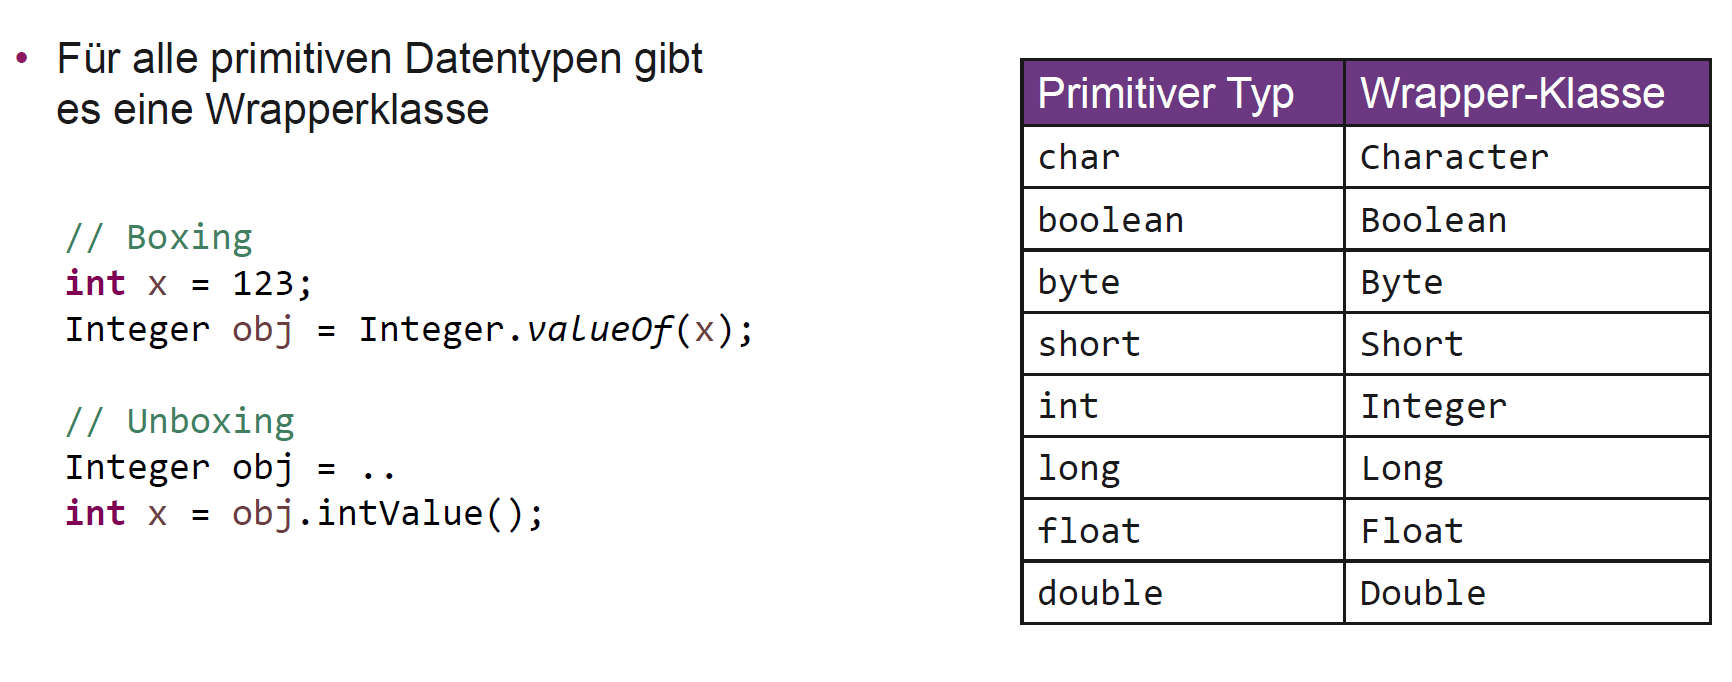
\includegraphics[width=0.9\columnwidth]{pictures/wrapper-klassen.png}
\end{center}

\subsection{ArrayList}
ArrayLists sind eine geordnete Folge von Elementen mit demselben Referenzdatentyp. Elemente können einfach 
hinzugefügt oder entfernt werden.\\
Der Zugriff auf Elemente erfolgt über Index (0 ... size()-1). Die Liste verwendet intern ein Array zur Verwaltung der Elemente.
Zu Beginn enthält sie, sofern nicht anders definiert, 10 Elemente und wird bei Erreichen der Kapazität mit Faktor 1.5 mulitpliziert.

\begin{center}
    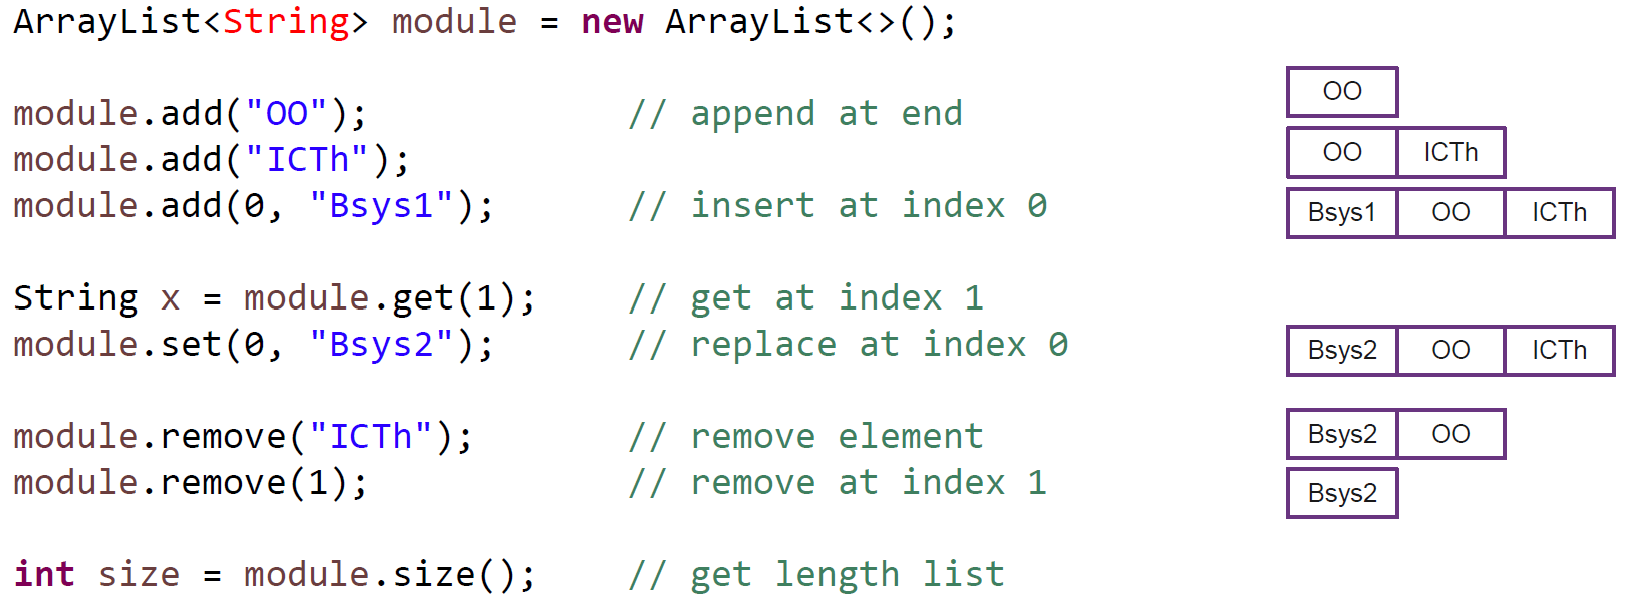
\includegraphics[width=0.9\columnwidth]{pictures/arrayList-bsp.png}
\end{center}

\begin{center}
    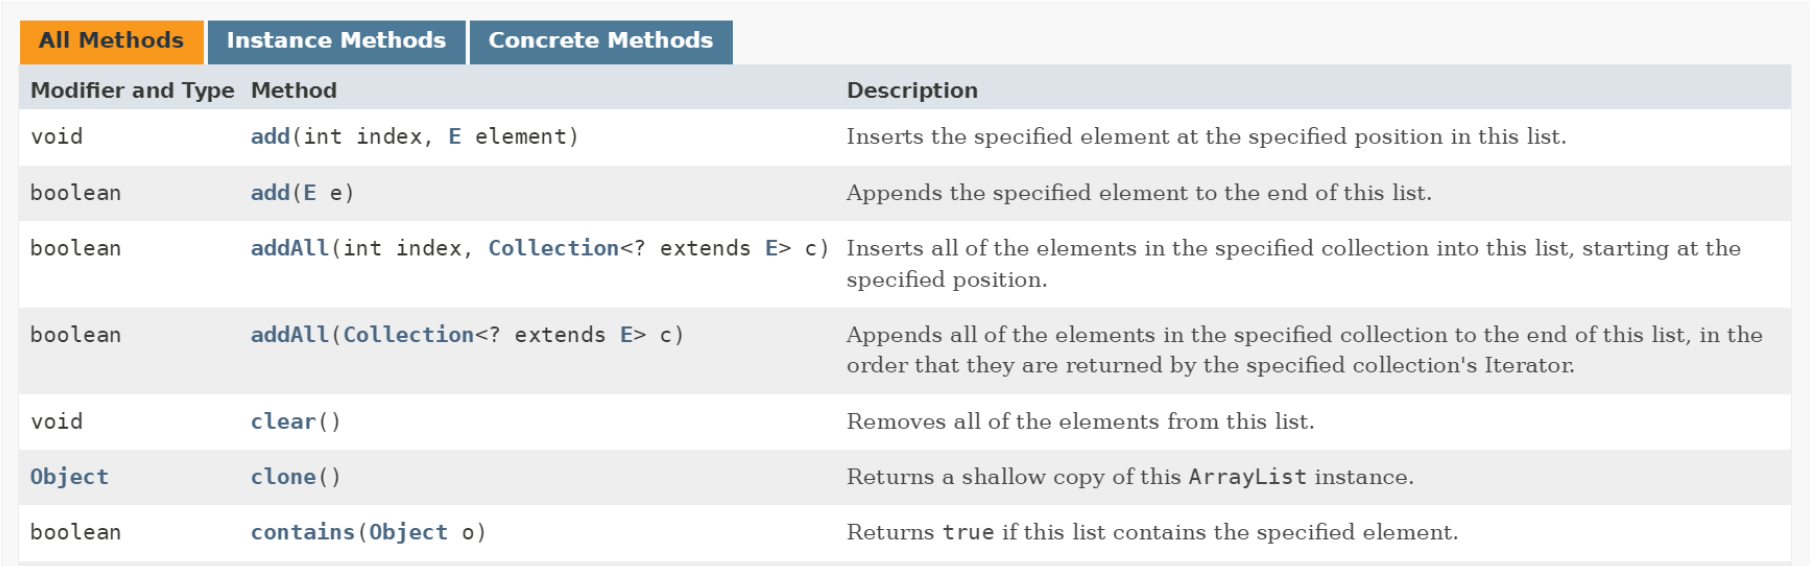
\includegraphics[width=0.9\columnwidth]{pictures/arrayList-api.png}
\end{center}

\subsection{LinkedList}

\subsection{HashSet}

\subsection{TreeSet}

\subsection{HashMap}

\subsection{TreeMap}
